\documentclass[twoside]{book}

% Packages required by doxygen
\usepackage{fixltx2e}
\usepackage{calc}
\usepackage{doxygen}
\usepackage[export]{adjustbox} % also loads graphicx
\usepackage{graphicx}
\usepackage[utf8]{inputenc}
\usepackage{makeidx}
\usepackage{multicol}
\usepackage{multirow}
\PassOptionsToPackage{warn}{textcomp}
\usepackage{textcomp}
\usepackage[nointegrals]{wasysym}
\usepackage[table]{xcolor}

% Font selection
\usepackage[T1]{fontenc}
\usepackage[scaled=.90]{helvet}
\usepackage{courier}
\usepackage{amssymb}
\usepackage{sectsty}
\renewcommand{\familydefault}{\sfdefault}
\allsectionsfont{%
  \fontseries{bc}\selectfont%
  \color{darkgray}%
}
\renewcommand{\DoxyLabelFont}{%
  \fontseries{bc}\selectfont%
  \color{darkgray}%
}
\newcommand{\+}{\discretionary{\mbox{\scriptsize$\hookleftarrow$}}{}{}}

% Page & text layout
\usepackage{geometry}
\geometry{%
  a4paper,%
  top=2.5cm,%
  bottom=2.5cm,%
  left=2.5cm,%
  right=2.5cm%
}
\tolerance=750
\hfuzz=15pt
\hbadness=750
\setlength{\emergencystretch}{15pt}
\setlength{\parindent}{0cm}
\setlength{\parskip}{3ex plus 2ex minus 2ex}
\makeatletter
\renewcommand{\paragraph}{%
  \@startsection{paragraph}{4}{0ex}{-1.0ex}{1.0ex}{%
    \normalfont\normalsize\bfseries\SS@parafont%
  }%
}
\renewcommand{\subparagraph}{%
  \@startsection{subparagraph}{5}{0ex}{-1.0ex}{1.0ex}{%
    \normalfont\normalsize\bfseries\SS@subparafont%
  }%
}
\makeatother

% Headers & footers
\usepackage{fancyhdr}
\pagestyle{fancyplain}
\fancyhead[LE]{\fancyplain{}{\bfseries\thepage}}
\fancyhead[CE]{\fancyplain{}{}}
\fancyhead[RE]{\fancyplain{}{\bfseries\leftmark}}
\fancyhead[LO]{\fancyplain{}{\bfseries\rightmark}}
\fancyhead[CO]{\fancyplain{}{}}
\fancyhead[RO]{\fancyplain{}{\bfseries\thepage}}
\fancyfoot[LE]{\fancyplain{}{}}
\fancyfoot[CE]{\fancyplain{}{}}
\fancyfoot[RE]{\fancyplain{}{\bfseries\scriptsize Generated by Doxygen }}
\fancyfoot[LO]{\fancyplain{}{\bfseries\scriptsize Generated by Doxygen }}
\fancyfoot[CO]{\fancyplain{}{}}
\fancyfoot[RO]{\fancyplain{}{}}
\renewcommand{\footrulewidth}{0.4pt}
\renewcommand{\chaptermark}[1]{%
  \markboth{#1}{}%
}
\renewcommand{\sectionmark}[1]{%
  \markright{\thesection\ #1}%
}

% Indices & bibliography
\usepackage{natbib}
\usepackage[titles]{tocloft}
\setcounter{tocdepth}{3}
\setcounter{secnumdepth}{5}
\makeindex

% Hyperlinks (required, but should be loaded last)
\usepackage{ifpdf}
\ifpdf
  \usepackage[pdftex,pagebackref=true]{hyperref}
\else
  \usepackage[ps2pdf,pagebackref=true]{hyperref}
\fi
\hypersetup{%
  colorlinks=true,%
  linkcolor=blue,%
  citecolor=blue,%
  unicode%
}

% Custom commands
\newcommand{\clearemptydoublepage}{%
  \newpage{\pagestyle{empty}\cleardoublepage}%
}

\usepackage{caption}
\captionsetup{labelsep=space,justification=centering,font={bf},singlelinecheck=off,skip=4pt,position=top}

%===== C O N T E N T S =====

\begin{document}

% Titlepage & ToC
\hypersetup{pageanchor=false,
             bookmarksnumbered=true,
             pdfencoding=unicode
            }
\pagenumbering{alph}
\begin{titlepage}
\vspace*{7cm}
\begin{center}%
{\Large My Project }\\
\vspace*{1cm}
{\large Generated by Doxygen 1.8.13}\\
\end{center}
\end{titlepage}
\clearemptydoublepage
\pagenumbering{roman}
\tableofcontents
\clearemptydoublepage
\pagenumbering{arabic}
\hypersetup{pageanchor=true}

%--- Begin generated contents ---
\chapter{Hierarchical Index}
\section{Class Hierarchy}
This inheritance list is sorted roughly, but not completely, alphabetically\+:\begin{DoxyCompactList}
\item Q\+Main\+Window\begin{DoxyCompactList}
\item \contentsline{section}{Main\+Window}{\pageref{classMainWindow}}{}
\end{DoxyCompactList}
\item Q\+Object\begin{DoxyCompactList}
\item \contentsline{section}{Backend\+Manual\+Tests\+Defferable\+Server}{\pageref{classBackendManualTestsDefferableServer}}{}
\item \contentsline{section}{Backend\+Manual\+Tests\+Polling\+Server}{\pageref{classBackendManualTestsPollingServer}}{}
\item \contentsline{section}{Controller}{\pageref{classController}}{}
\end{DoxyCompactList}
\end{DoxyCompactList}

\chapter{Class Index}
\section{Class List}
Here are the classes, structs, unions and interfaces with brief descriptions\+:\begin{DoxyCompactList}
\item\contentsline{section}{\hyperlink{classBackendManualTestsDefferableServer}{Backend\+Manual\+Tests\+Defferable\+Server} }{\pageref{classBackendManualTestsDefferableServer}}{}
\item\contentsline{section}{\hyperlink{classBackendManualTestsPollingServer}{Backend\+Manual\+Tests\+Polling\+Server} }{\pageref{classBackendManualTestsPollingServer}}{}
\item\contentsline{section}{\hyperlink{classController}{Controller} }{\pageref{classController}}{}
\item\contentsline{section}{\hyperlink{classMainWindow}{Main\+Window} }{\pageref{classMainWindow}}{}
\end{DoxyCompactList}

\chapter{Class Documentation}
\hypertarget{classBackendManualTestsDefferableServer}{}\section{Backend\+Manual\+Tests\+Defferable\+Server Class Reference}
\label{classBackendManualTestsDefferableServer}\index{Backend\+Manual\+Tests\+Defferable\+Server@{Backend\+Manual\+Tests\+Defferable\+Server}}


Inheritance diagram for Backend\+Manual\+Tests\+Defferable\+Server\+:\nopagebreak
\begin{figure}[H]
\begin{center}
\leavevmode
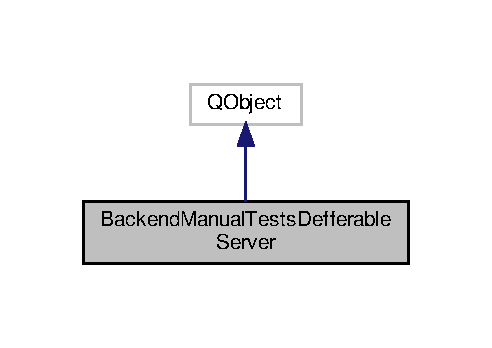
\includegraphics[width=236pt]{classBackendManualTestsDefferableServer__inherit__graph}
\end{center}
\end{figure}


Collaboration diagram for Backend\+Manual\+Tests\+Defferable\+Server\+:\nopagebreak
\begin{figure}[H]
\begin{center}
\leavevmode
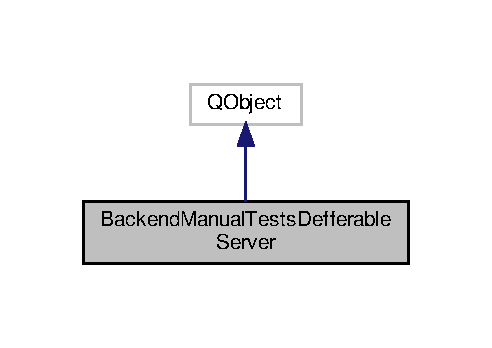
\includegraphics[width=236pt]{classBackendManualTestsDefferableServer__coll__graph}
\end{center}
\end{figure}
\subsection*{Public Member Functions}
\begin{DoxyCompactItemize}
\item 
\mbox{\Hypertarget{classBackendManualTestsDefferableServer_a3c6facaeee8515a5f9146681eb66d30c}\label{classBackendManualTestsDefferableServer_a3c6facaeee8515a5f9146681eb66d30c}} 
{\bfseries Backend\+Manual\+Tests\+Defferable\+Server} (Q\+Object $\ast$parent=nullptr)
\end{DoxyCompactItemize}


The documentation for this class was generated from the following files\+:\begin{DoxyCompactItemize}
\item 
backendmanualtestsdefferableserver.\+h\item 
backendmanualtestsdefferableserver.\+cpp\end{DoxyCompactItemize}

\hypertarget{classBackendManualTestsPollingServer}{}\section{Backend\+Manual\+Tests\+Polling\+Server Class Reference}
\label{classBackendManualTestsPollingServer}\index{Backend\+Manual\+Tests\+Polling\+Server@{Backend\+Manual\+Tests\+Polling\+Server}}


Inheritance diagram for Backend\+Manual\+Tests\+Polling\+Server\+:\nopagebreak
\begin{figure}[H]
\begin{center}
\leavevmode
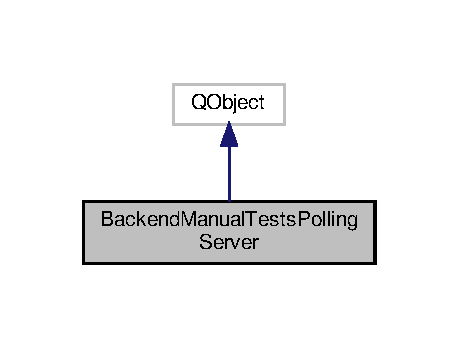
\includegraphics[width=220pt]{classBackendManualTestsPollingServer__inherit__graph}
\end{center}
\end{figure}


Collaboration diagram for Backend\+Manual\+Tests\+Polling\+Server\+:\nopagebreak
\begin{figure}[H]
\begin{center}
\leavevmode
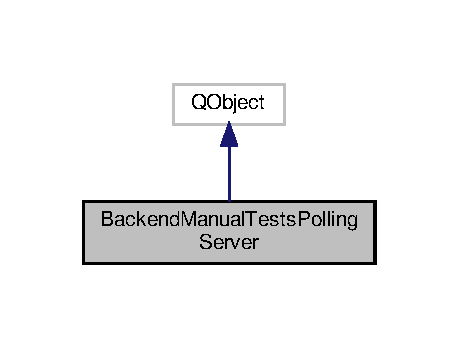
\includegraphics[width=220pt]{classBackendManualTestsPollingServer__coll__graph}
\end{center}
\end{figure}
\subsection*{Public Member Functions}
\begin{DoxyCompactItemize}
\item 
\mbox{\Hypertarget{classBackendManualTestsPollingServer_aa1b870718edee843e64807451ff41dea}\label{classBackendManualTestsPollingServer_aa1b870718edee843e64807451ff41dea}} 
{\bfseries Backend\+Manual\+Tests\+Polling\+Server} (Q\+Object $\ast$parent)
\end{DoxyCompactItemize}
\subsection*{Static Public Member Functions}
\begin{DoxyCompactItemize}
\item 
\mbox{\Hypertarget{classBackendManualTestsPollingServer_af4380e1a4fd0bafc6d47093f05d37e59}\label{classBackendManualTestsPollingServer_af4380e1a4fd0bafc6d47093f05d37e59}} 
static int $\ast$ {\bfseries generate\+\_\+schedule} (int $\ast$size, Q\+String filename)
\item 
\mbox{\Hypertarget{classBackendManualTestsPollingServer_a093c578eacbe839ce1bafc1e907d53f9}\label{classBackendManualTestsPollingServer_a093c578eacbe839ce1bafc1e907d53f9}} 
static bool {\bfseries results} (Aperiodic\+Scheduler $\ast$ps, int len, int $\ast$sched, bool expected, int i, int $\ast$finish\+\_\+times)
\item 
\mbox{\Hypertarget{classBackendManualTestsPollingServer_ac4f8b7a094f44fa42428206db0d0bdd5}\label{classBackendManualTestsPollingServer_ac4f8b7a094f44fa42428206db0d0bdd5}} 
static Q\+String {\bfseries result\+\_\+messages} (int i)
\end{DoxyCompactItemize}


The documentation for this class was generated from the following files\+:\begin{DoxyCompactItemize}
\item 
backendmanualtestspollingserver.\+h\item 
backendmanualtestspollingserver.\+cpp\end{DoxyCompactItemize}

\hypertarget{classController}{}\section{Controller Class Reference}
\label{classController}\index{Controller@{Controller}}


Inheritance diagram for Controller\+:\nopagebreak
\begin{figure}[H]
\begin{center}
\leavevmode
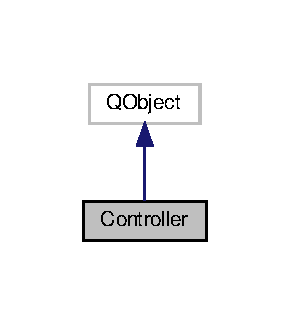
\includegraphics[width=139pt]{classController__inherit__graph}
\end{center}
\end{figure}


Collaboration diagram for Controller\+:\nopagebreak
\begin{figure}[H]
\begin{center}
\leavevmode
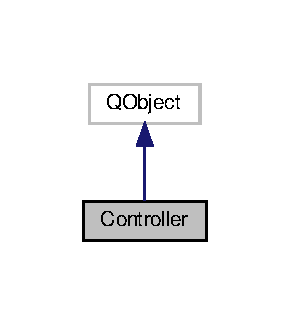
\includegraphics[width=139pt]{classController__coll__graph}
\end{center}
\end{figure}
\subsection*{Public Slots}
\begin{DoxyCompactItemize}
\item 
void \hyperlink{classController_a7db4c90e6055889682d8521f48c693f6}{file\+\_\+input\+\_\+selected} (bool checked)
\begin{DoxyCompactList}\small\item\em \hyperlink{classController_a7db4c90e6055889682d8521f48c693f6}{Controller\+::file\+\_\+input\+\_\+selected} This is a slot that is mapped to the file input button. This will execute upon pressing the file input button. It will try to read from the files currently in the input window. \end{DoxyCompactList}\item 
void \hyperlink{classController_a2daeb91e3a6c79ddfa46fd04770012ff}{manual\+\_\+input\+\_\+selected} (bool checked)
\begin{DoxyCompactList}\small\item\em \hyperlink{classController_a2daeb91e3a6c79ddfa46fd04770012ff}{Controller\+::manual\+\_\+input\+\_\+selected} This slot will launch a manual output subwindow based on the number of tasks inputted by the user. It is triggered by the manual input button in the mainwindow. \end{DoxyCompactList}\item 
void \hyperlink{classController_aeca721bb54b3495d2a490d6f658799a5}{polling\+\_\+server\+\_\+selected} (bool checked)
\begin{DoxyCompactList}\small\item\em \hyperlink{classController_aeca721bb54b3495d2a490d6f658799a5}{Controller\+::polling\+\_\+server\+\_\+selected} This is a slot mapped to the pollingserver checkbox in the analysis window. When the polling server box is checked it will lock the field until run\+\_\+analysis button or polling server is unclicked. \end{DoxyCompactList}\item 
void \hyperlink{classController_a1c4186c6a1366dc848cdeb68261dc12e}{defferable\+\_\+server\+\_\+selected} (bool checked)
\begin{DoxyCompactList}\small\item\em \hyperlink{classController_a1c4186c6a1366dc848cdeb68261dc12e}{Controller\+::defferable\+\_\+server\+\_\+selected} This is another slot with the same function as \hyperlink{classController_aeca721bb54b3495d2a490d6f658799a5}{polling\+\_\+server\+\_\+selected()}, except for defferable server. \end{DoxyCompactList}\item 
void \hyperlink{classController_ac9238da3e2cdd53dbc2a08cf9a55d4d2}{cpu\+\_\+selected} (bool checked)
\begin{DoxyCompactList}\small\item\em \hyperlink{classController_ac9238da3e2cdd53dbc2a08cf9a55d4d2}{Controller\+::cpu\+\_\+selected} This is a slot that is mapped to the cpu checkbox in the Analysis\+Window class. \end{DoxyCompactList}\item 
void \hyperlink{classController_a1573db92761b7e61b6dcace9c97aebf5}{context\+\_\+selected} (bool checked)
\begin{DoxyCompactList}\small\item\em \hyperlink{classController_a1573db92761b7e61b6dcace9c97aebf5}{Controller\+::context\+\_\+selected} This is a slot that is mapped to the context switch checkbox in the Analysis\+Window class. \end{DoxyCompactList}\item 
void \hyperlink{classController_a04531b0d9ee8f02677b1a562a2607ada}{response\+\_\+selected} (bool checked)
\begin{DoxyCompactList}\small\item\em \hyperlink{classController_a04531b0d9ee8f02677b1a562a2607ada}{Controller\+::response\+\_\+selected} This is a slot that is mapped to the avg response time checkbox in the Analysis\+Window class. \end{DoxyCompactList}\item 
void \hyperlink{classController_a7ff7d2d0e8614494020bf5e35dc663a8}{run\+\_\+analysis} (bool checked)
\begin{DoxyCompactList}\small\item\em \hyperlink{classController_a7ff7d2d0e8614494020bf5e35dc663a8}{Controller\+::run\+\_\+analysis} This is a slot that is mapped to the run analysis button in the Analysis\+Window. It will check all the flags of the controller class to check for a valid run configuration. If the run configuration is valid it will generate an Aperiodic\+Scheduler object and populate the graph display window at the top of the mainwindow. It will also compute any checked analysis metrics. \end{DoxyCompactList}\item 
\mbox{\Hypertarget{classController_a115dc63f10237164d2da71a0a0b6cf88}\label{classController_a115dc63f10237164d2da71a0a0b6cf88}} 
void {\bfseries update\+\_\+zoom\+\_\+level} ()
\item 
void \hyperlink{classController_aeec075efe687085d150d1e47504485c2}{open\+\_\+seperate\+\_\+schedule} (bool checked)
\begin{DoxyCompactList}\small\item\em \hyperlink{classController_aeec075efe687085d150d1e47504485c2}{Controller\+::open\+\_\+seperate\+\_\+schedule} This slot is mapped to the open\+\_\+seperate\+\_\+window button of the Display\+Adjuster Window. This opens a seperate graph display window, because it is hard to view sometimes with large schedules. \end{DoxyCompactList}\item 
\mbox{\Hypertarget{classController_a5cc451d3dd99282686381c3ff4e06e8a}\label{classController_a5cc451d3dd99282686381c3ff4e06e8a}} 
void \hyperlink{classController_a5cc451d3dd99282686381c3ff4e06e8a}{update\+\_\+start\+\_\+time} ()
\begin{DoxyCompactList}\small\item\em \hyperlink{classController_a5cc451d3dd99282686381c3ff4e06e8a}{Controller\+::update\+\_\+start\+\_\+time} This sets the left bound for the Graph\+Display Window. \end{DoxyCompactList}\item 
\mbox{\Hypertarget{classController_a9342c31418f227c4ab532bcc060ced7b}\label{classController_a9342c31418f227c4ab532bcc060ced7b}} 
void \hyperlink{classController_a9342c31418f227c4ab532bcc060ced7b}{update\+\_\+end\+\_\+time} ()
\begin{DoxyCompactList}\small\item\em \hyperlink{classController_a9342c31418f227c4ab532bcc060ced7b}{Controller\+::update\+\_\+end\+\_\+time} This slot sets the right bound for the Graph\+Display Window. \end{DoxyCompactList}\end{DoxyCompactItemize}
\subsection*{Public Member Functions}
\begin{DoxyCompactItemize}
\item 
\hyperlink{classController_ac162dc9f74ef4ba011d7026b803c4f12}{Controller} (Q\+Object $\ast$parent=nullptr, Workload\+Window $\ast$workload\+\_\+window=nullptr, Analysis\+Window $\ast$analysis\+\_\+window=nullptr, Display\+Adjuster $\ast$display\+\_\+adjuster=nullptr, Graph\+Display $\ast$graph\+\_\+display=nullptr)
\begin{DoxyCompactList}\small\item\em \hyperlink{classController_ac162dc9f74ef4ba011d7026b803c4f12}{Controller\+::\+Controller} This Class is used for routing information in Frontend=$>$Frontend and Frontend=$>$Backend Communication. \end{DoxyCompactList}\item 
\mbox{\Hypertarget{classController_a26511d6997388ccfe8f5ae02d49d9e6e}\label{classController_a26511d6997388ccfe8f5ae02d49d9e6e}} 
void \hyperlink{classController_a26511d6997388ccfe8f5ae02d49d9e6e}{connect\+\_\+sigs} ()
\begin{DoxyCompactList}\small\item\em \hyperlink{classController_a26511d6997388ccfe8f5ae02d49d9e6e}{Controller\+::connect\+\_\+sigs} This function is called in the constructor to Map all the slots and signals of the subwindows of the mainwindow. \end{DoxyCompactList}\item 
\mbox{\Hypertarget{classController_a57bd1103e450b49bfbbf452ab401c720}\label{classController_a57bd1103e450b49bfbbf452ab401c720}} 
void {\bfseries set\+Schedule} (int $\ast$value)
\end{DoxyCompactItemize}


\subsection{Constructor \& Destructor Documentation}
\mbox{\Hypertarget{classController_ac162dc9f74ef4ba011d7026b803c4f12}\label{classController_ac162dc9f74ef4ba011d7026b803c4f12}} 
\index{Controller@{Controller}!Controller@{Controller}}
\index{Controller@{Controller}!Controller@{Controller}}
\subsubsection{\texorpdfstring{Controller()}{Controller()}}
{\footnotesize\ttfamily Controller\+::\+Controller (\begin{DoxyParamCaption}\item[{Q\+Object $\ast$}]{parent = {\ttfamily nullptr},  }\item[{Workload\+Window $\ast$}]{workload\+\_\+window = {\ttfamily nullptr},  }\item[{Analysis\+Window $\ast$}]{analysis\+\_\+window = {\ttfamily nullptr},  }\item[{Display\+Adjuster $\ast$}]{display\+\_\+adjuster = {\ttfamily nullptr},  }\item[{Graph\+Display $\ast$}]{graph\+\_\+display = {\ttfamily nullptr} }\end{DoxyParamCaption})\hspace{0.3cm}{\ttfamily [explicit]}}



\hyperlink{classController_ac162dc9f74ef4ba011d7026b803c4f12}{Controller\+::\+Controller} This Class is used for routing information in Frontend=$>$Frontend and Frontend=$>$Backend Communication. 


\begin{DoxyParams}{Parameters}
{\em parent} & Not used \\
\hline
\end{DoxyParams}


\subsection{Member Function Documentation}
\mbox{\Hypertarget{classController_a1573db92761b7e61b6dcace9c97aebf5}\label{classController_a1573db92761b7e61b6dcace9c97aebf5}} 
\index{Controller@{Controller}!context\+\_\+selected@{context\+\_\+selected}}
\index{context\+\_\+selected@{context\+\_\+selected}!Controller@{Controller}}
\subsubsection{\texorpdfstring{context\+\_\+selected}{context\_selected}}
{\footnotesize\ttfamily void Controller\+::context\+\_\+selected (\begin{DoxyParamCaption}\item[{bool}]{checked }\end{DoxyParamCaption})\hspace{0.3cm}{\ttfamily [slot]}}



\hyperlink{classController_a1573db92761b7e61b6dcace9c97aebf5}{Controller\+::context\+\_\+selected} This is a slot that is mapped to the context switch checkbox in the Analysis\+Window class. 


\begin{DoxyParams}{Parameters}
{\em checked} & \\
\hline
\end{DoxyParams}
\mbox{\Hypertarget{classController_ac9238da3e2cdd53dbc2a08cf9a55d4d2}\label{classController_ac9238da3e2cdd53dbc2a08cf9a55d4d2}} 
\index{Controller@{Controller}!cpu\+\_\+selected@{cpu\+\_\+selected}}
\index{cpu\+\_\+selected@{cpu\+\_\+selected}!Controller@{Controller}}
\subsubsection{\texorpdfstring{cpu\+\_\+selected}{cpu\_selected}}
{\footnotesize\ttfamily void Controller\+::cpu\+\_\+selected (\begin{DoxyParamCaption}\item[{bool}]{checked }\end{DoxyParamCaption})\hspace{0.3cm}{\ttfamily [slot]}}



\hyperlink{classController_ac9238da3e2cdd53dbc2a08cf9a55d4d2}{Controller\+::cpu\+\_\+selected} This is a slot that is mapped to the cpu checkbox in the Analysis\+Window class. 


\begin{DoxyParams}{Parameters}
{\em checked} & \\
\hline
\end{DoxyParams}
\mbox{\Hypertarget{classController_a1c4186c6a1366dc848cdeb68261dc12e}\label{classController_a1c4186c6a1366dc848cdeb68261dc12e}} 
\index{Controller@{Controller}!defferable\+\_\+server\+\_\+selected@{defferable\+\_\+server\+\_\+selected}}
\index{defferable\+\_\+server\+\_\+selected@{defferable\+\_\+server\+\_\+selected}!Controller@{Controller}}
\subsubsection{\texorpdfstring{defferable\+\_\+server\+\_\+selected}{defferable\_server\_selected}}
{\footnotesize\ttfamily void Controller\+::defferable\+\_\+server\+\_\+selected (\begin{DoxyParamCaption}\item[{bool}]{checked }\end{DoxyParamCaption})\hspace{0.3cm}{\ttfamily [slot]}}



\hyperlink{classController_a1c4186c6a1366dc848cdeb68261dc12e}{Controller\+::defferable\+\_\+server\+\_\+selected} This is another slot with the same function as \hyperlink{classController_aeca721bb54b3495d2a490d6f658799a5}{polling\+\_\+server\+\_\+selected()}, except for defferable server. 


\begin{DoxyParams}{Parameters}
{\em checked} & \\
\hline
\end{DoxyParams}
\mbox{\Hypertarget{classController_a7db4c90e6055889682d8521f48c693f6}\label{classController_a7db4c90e6055889682d8521f48c693f6}} 
\index{Controller@{Controller}!file\+\_\+input\+\_\+selected@{file\+\_\+input\+\_\+selected}}
\index{file\+\_\+input\+\_\+selected@{file\+\_\+input\+\_\+selected}!Controller@{Controller}}
\subsubsection{\texorpdfstring{file\+\_\+input\+\_\+selected}{file\_input\_selected}}
{\footnotesize\ttfamily void Controller\+::file\+\_\+input\+\_\+selected (\begin{DoxyParamCaption}\item[{bool}]{checked }\end{DoxyParamCaption})\hspace{0.3cm}{\ttfamily [slot]}}



\hyperlink{classController_a7db4c90e6055889682d8521f48c693f6}{Controller\+::file\+\_\+input\+\_\+selected} This is a slot that is mapped to the file input button. This will execute upon pressing the file input button. It will try to read from the files currently in the input window. 


\begin{DoxyParams}{Parameters}
{\em checked} & \\
\hline
\end{DoxyParams}
\mbox{\Hypertarget{classController_a2daeb91e3a6c79ddfa46fd04770012ff}\label{classController_a2daeb91e3a6c79ddfa46fd04770012ff}} 
\index{Controller@{Controller}!manual\+\_\+input\+\_\+selected@{manual\+\_\+input\+\_\+selected}}
\index{manual\+\_\+input\+\_\+selected@{manual\+\_\+input\+\_\+selected}!Controller@{Controller}}
\subsubsection{\texorpdfstring{manual\+\_\+input\+\_\+selected}{manual\_input\_selected}}
{\footnotesize\ttfamily void Controller\+::manual\+\_\+input\+\_\+selected (\begin{DoxyParamCaption}\item[{bool}]{checked }\end{DoxyParamCaption})\hspace{0.3cm}{\ttfamily [slot]}}



\hyperlink{classController_a2daeb91e3a6c79ddfa46fd04770012ff}{Controller\+::manual\+\_\+input\+\_\+selected} This slot will launch a manual output subwindow based on the number of tasks inputted by the user. It is triggered by the manual input button in the mainwindow. 


\begin{DoxyParams}{Parameters}
{\em checked} & \\
\hline
\end{DoxyParams}
\mbox{\Hypertarget{classController_aeec075efe687085d150d1e47504485c2}\label{classController_aeec075efe687085d150d1e47504485c2}} 
\index{Controller@{Controller}!open\+\_\+seperate\+\_\+schedule@{open\+\_\+seperate\+\_\+schedule}}
\index{open\+\_\+seperate\+\_\+schedule@{open\+\_\+seperate\+\_\+schedule}!Controller@{Controller}}
\subsubsection{\texorpdfstring{open\+\_\+seperate\+\_\+schedule}{open\_seperate\_schedule}}
{\footnotesize\ttfamily void Controller\+::open\+\_\+seperate\+\_\+schedule (\begin{DoxyParamCaption}\item[{bool}]{checked }\end{DoxyParamCaption})\hspace{0.3cm}{\ttfamily [slot]}}



\hyperlink{classController_aeec075efe687085d150d1e47504485c2}{Controller\+::open\+\_\+seperate\+\_\+schedule} This slot is mapped to the open\+\_\+seperate\+\_\+window button of the Display\+Adjuster Window. This opens a seperate graph display window, because it is hard to view sometimes with large schedules. 


\begin{DoxyParams}{Parameters}
{\em checked} & \\
\hline
\end{DoxyParams}
\mbox{\Hypertarget{classController_aeca721bb54b3495d2a490d6f658799a5}\label{classController_aeca721bb54b3495d2a490d6f658799a5}} 
\index{Controller@{Controller}!polling\+\_\+server\+\_\+selected@{polling\+\_\+server\+\_\+selected}}
\index{polling\+\_\+server\+\_\+selected@{polling\+\_\+server\+\_\+selected}!Controller@{Controller}}
\subsubsection{\texorpdfstring{polling\+\_\+server\+\_\+selected}{polling\_server\_selected}}
{\footnotesize\ttfamily void Controller\+::polling\+\_\+server\+\_\+selected (\begin{DoxyParamCaption}\item[{bool}]{checked }\end{DoxyParamCaption})\hspace{0.3cm}{\ttfamily [slot]}}



\hyperlink{classController_aeca721bb54b3495d2a490d6f658799a5}{Controller\+::polling\+\_\+server\+\_\+selected} This is a slot mapped to the pollingserver checkbox in the analysis window. When the polling server box is checked it will lock the field until run\+\_\+analysis button or polling server is unclicked. 


\begin{DoxyParams}{Parameters}
{\em checked} & \\
\hline
\end{DoxyParams}
\mbox{\Hypertarget{classController_a04531b0d9ee8f02677b1a562a2607ada}\label{classController_a04531b0d9ee8f02677b1a562a2607ada}} 
\index{Controller@{Controller}!response\+\_\+selected@{response\+\_\+selected}}
\index{response\+\_\+selected@{response\+\_\+selected}!Controller@{Controller}}
\subsubsection{\texorpdfstring{response\+\_\+selected}{response\_selected}}
{\footnotesize\ttfamily void Controller\+::response\+\_\+selected (\begin{DoxyParamCaption}\item[{bool}]{checked }\end{DoxyParamCaption})\hspace{0.3cm}{\ttfamily [slot]}}



\hyperlink{classController_a04531b0d9ee8f02677b1a562a2607ada}{Controller\+::response\+\_\+selected} This is a slot that is mapped to the avg response time checkbox in the Analysis\+Window class. 


\begin{DoxyParams}{Parameters}
{\em checked} & \\
\hline
\end{DoxyParams}
\mbox{\Hypertarget{classController_a7ff7d2d0e8614494020bf5e35dc663a8}\label{classController_a7ff7d2d0e8614494020bf5e35dc663a8}} 
\index{Controller@{Controller}!run\+\_\+analysis@{run\+\_\+analysis}}
\index{run\+\_\+analysis@{run\+\_\+analysis}!Controller@{Controller}}
\subsubsection{\texorpdfstring{run\+\_\+analysis}{run\_analysis}}
{\footnotesize\ttfamily void Controller\+::run\+\_\+analysis (\begin{DoxyParamCaption}\item[{bool}]{checked }\end{DoxyParamCaption})\hspace{0.3cm}{\ttfamily [slot]}}



\hyperlink{classController_a7ff7d2d0e8614494020bf5e35dc663a8}{Controller\+::run\+\_\+analysis} This is a slot that is mapped to the run analysis button in the Analysis\+Window. It will check all the flags of the controller class to check for a valid run configuration. If the run configuration is valid it will generate an Aperiodic\+Scheduler object and populate the graph display window at the top of the mainwindow. It will also compute any checked analysis metrics. 


\begin{DoxyParams}{Parameters}
{\em checked} & \\
\hline
\end{DoxyParams}


The documentation for this class was generated from the following files\+:\begin{DoxyCompactItemize}
\item 
controller.\+h\item 
controller.\+cpp\end{DoxyCompactItemize}

\hypertarget{classMainWindow}{}\section{Main\+Window Class Reference}
\label{classMainWindow}\index{Main\+Window@{Main\+Window}}


Inheritance diagram for Main\+Window\+:\nopagebreak
\begin{figure}[H]
\begin{center}
\leavevmode
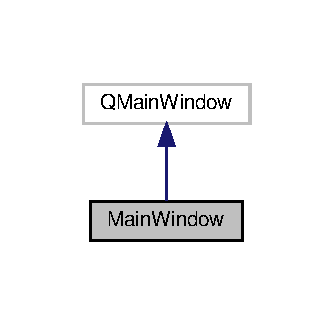
\includegraphics[width=160pt]{classMainWindow__inherit__graph}
\end{center}
\end{figure}


Collaboration diagram for Main\+Window\+:\nopagebreak
\begin{figure}[H]
\begin{center}
\leavevmode
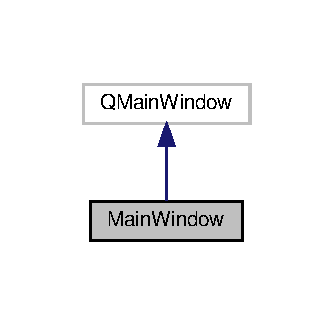
\includegraphics[width=160pt]{classMainWindow__coll__graph}
\end{center}
\end{figure}
\subsection*{Public Member Functions}
\begin{DoxyCompactItemize}
\item 
\hyperlink{classMainWindow_a6f640c3030f6a8fafe1a70585e8db0ea}{Main\+Window} (Q\+Widget $\ast$parent=nullptr, Q\+Widget $\ast$schedule\+\_\+panel=nullptr, Workload\+Window $\ast$workload\+\_\+panel=nullptr, Q\+Widget $\ast$analysis\+\_\+panel=nullptr, Q\+Widget $\ast$display\+\_\+adjuster=nullptr, Q\+Object $\ast$controller=nullptr)
\begin{DoxyCompactList}\small\item\em \hyperlink{classMainWindow_a6f640c3030f6a8fafe1a70585e8db0ea}{Main\+Window\+::\+Main\+Window} This is the standard constructor for my main window widget. It populates the empty scroll areas in the main with the four child widgets of the app. \end{DoxyCompactList}\end{DoxyCompactItemize}


\subsection{Constructor \& Destructor Documentation}
\mbox{\Hypertarget{classMainWindow_a6f640c3030f6a8fafe1a70585e8db0ea}\label{classMainWindow_a6f640c3030f6a8fafe1a70585e8db0ea}} 
\index{Main\+Window@{Main\+Window}!Main\+Window@{Main\+Window}}
\index{Main\+Window@{Main\+Window}!Main\+Window@{Main\+Window}}
\subsubsection{\texorpdfstring{Main\+Window()}{MainWindow()}}
{\footnotesize\ttfamily Main\+Window\+::\+Main\+Window (\begin{DoxyParamCaption}\item[{Q\+Widget $\ast$}]{parent = {\ttfamily nullptr},  }\item[{Q\+Widget $\ast$}]{schedule\+\_\+panel = {\ttfamily nullptr},  }\item[{Workload\+Window $\ast$}]{workload\+\_\+panel = {\ttfamily nullptr},  }\item[{Q\+Widget $\ast$}]{analysis\+\_\+panel = {\ttfamily nullptr},  }\item[{Q\+Widget $\ast$}]{display\+\_\+adjuster = {\ttfamily nullptr},  }\item[{Q\+Object $\ast$}]{controller = {\ttfamily nullptr} }\end{DoxyParamCaption})}



\hyperlink{classMainWindow_a6f640c3030f6a8fafe1a70585e8db0ea}{Main\+Window\+::\+Main\+Window} This is the standard constructor for my main window widget. It populates the empty scroll areas in the main with the four child widgets of the app. 


\begin{DoxyParams}{Parameters}
{\em parent} & This is the parent widget. It is not used. \\
\hline
{\em schedule\+\_\+panel} & This is the schedule panel widget. This is a graph generated by Qpainter. \\
\hline
{\em workload\+\_\+panel} & This is the workload panel. This panel allows a user to specify the properties of the periodic and aperiodic workloads by supplying input files or manually inputting values. \\
\hline
{\em analysis\+\_\+panel} & This is the analysis panel. There are G\+UI elements in this widget that allow a user to specify what types of properties they want to observe \\
\hline
{\em display\+\_\+adjuster} & This panel is used for adjusting the display of the schedule\+\_\+panel. It allows a user to zoom and specify time bounds to display. \\
\hline
{\em controller} & This object controls all the widgets. It reads signals from widgets and routes the information to the other panels. \\
\hline
\end{DoxyParams}


The documentation for this class was generated from the following files\+:\begin{DoxyCompactItemize}
\item 
mainwindow.\+h\item 
mainwindow.\+cpp\end{DoxyCompactItemize}

%--- End generated contents ---

% Index
\backmatter
\newpage
\phantomsection
\clearemptydoublepage
\addcontentsline{toc}{chapter}{Index}
\printindex

\end{document}
